\documentclass[12pt]{article}

\usepackage{graphicx}
\graphicspath{ {Fichier_Image/} }

\title{Hypothèses}
\author{Thibault Clodion}

\begin{document}

\maketitle % Permet d'afficher le titre, l'author etc

L'objectif est ici de réaliser un bâtiment dont le temps de sortie est minimale tout en 
respectant le CDC n°1.

\section{Création Générale}

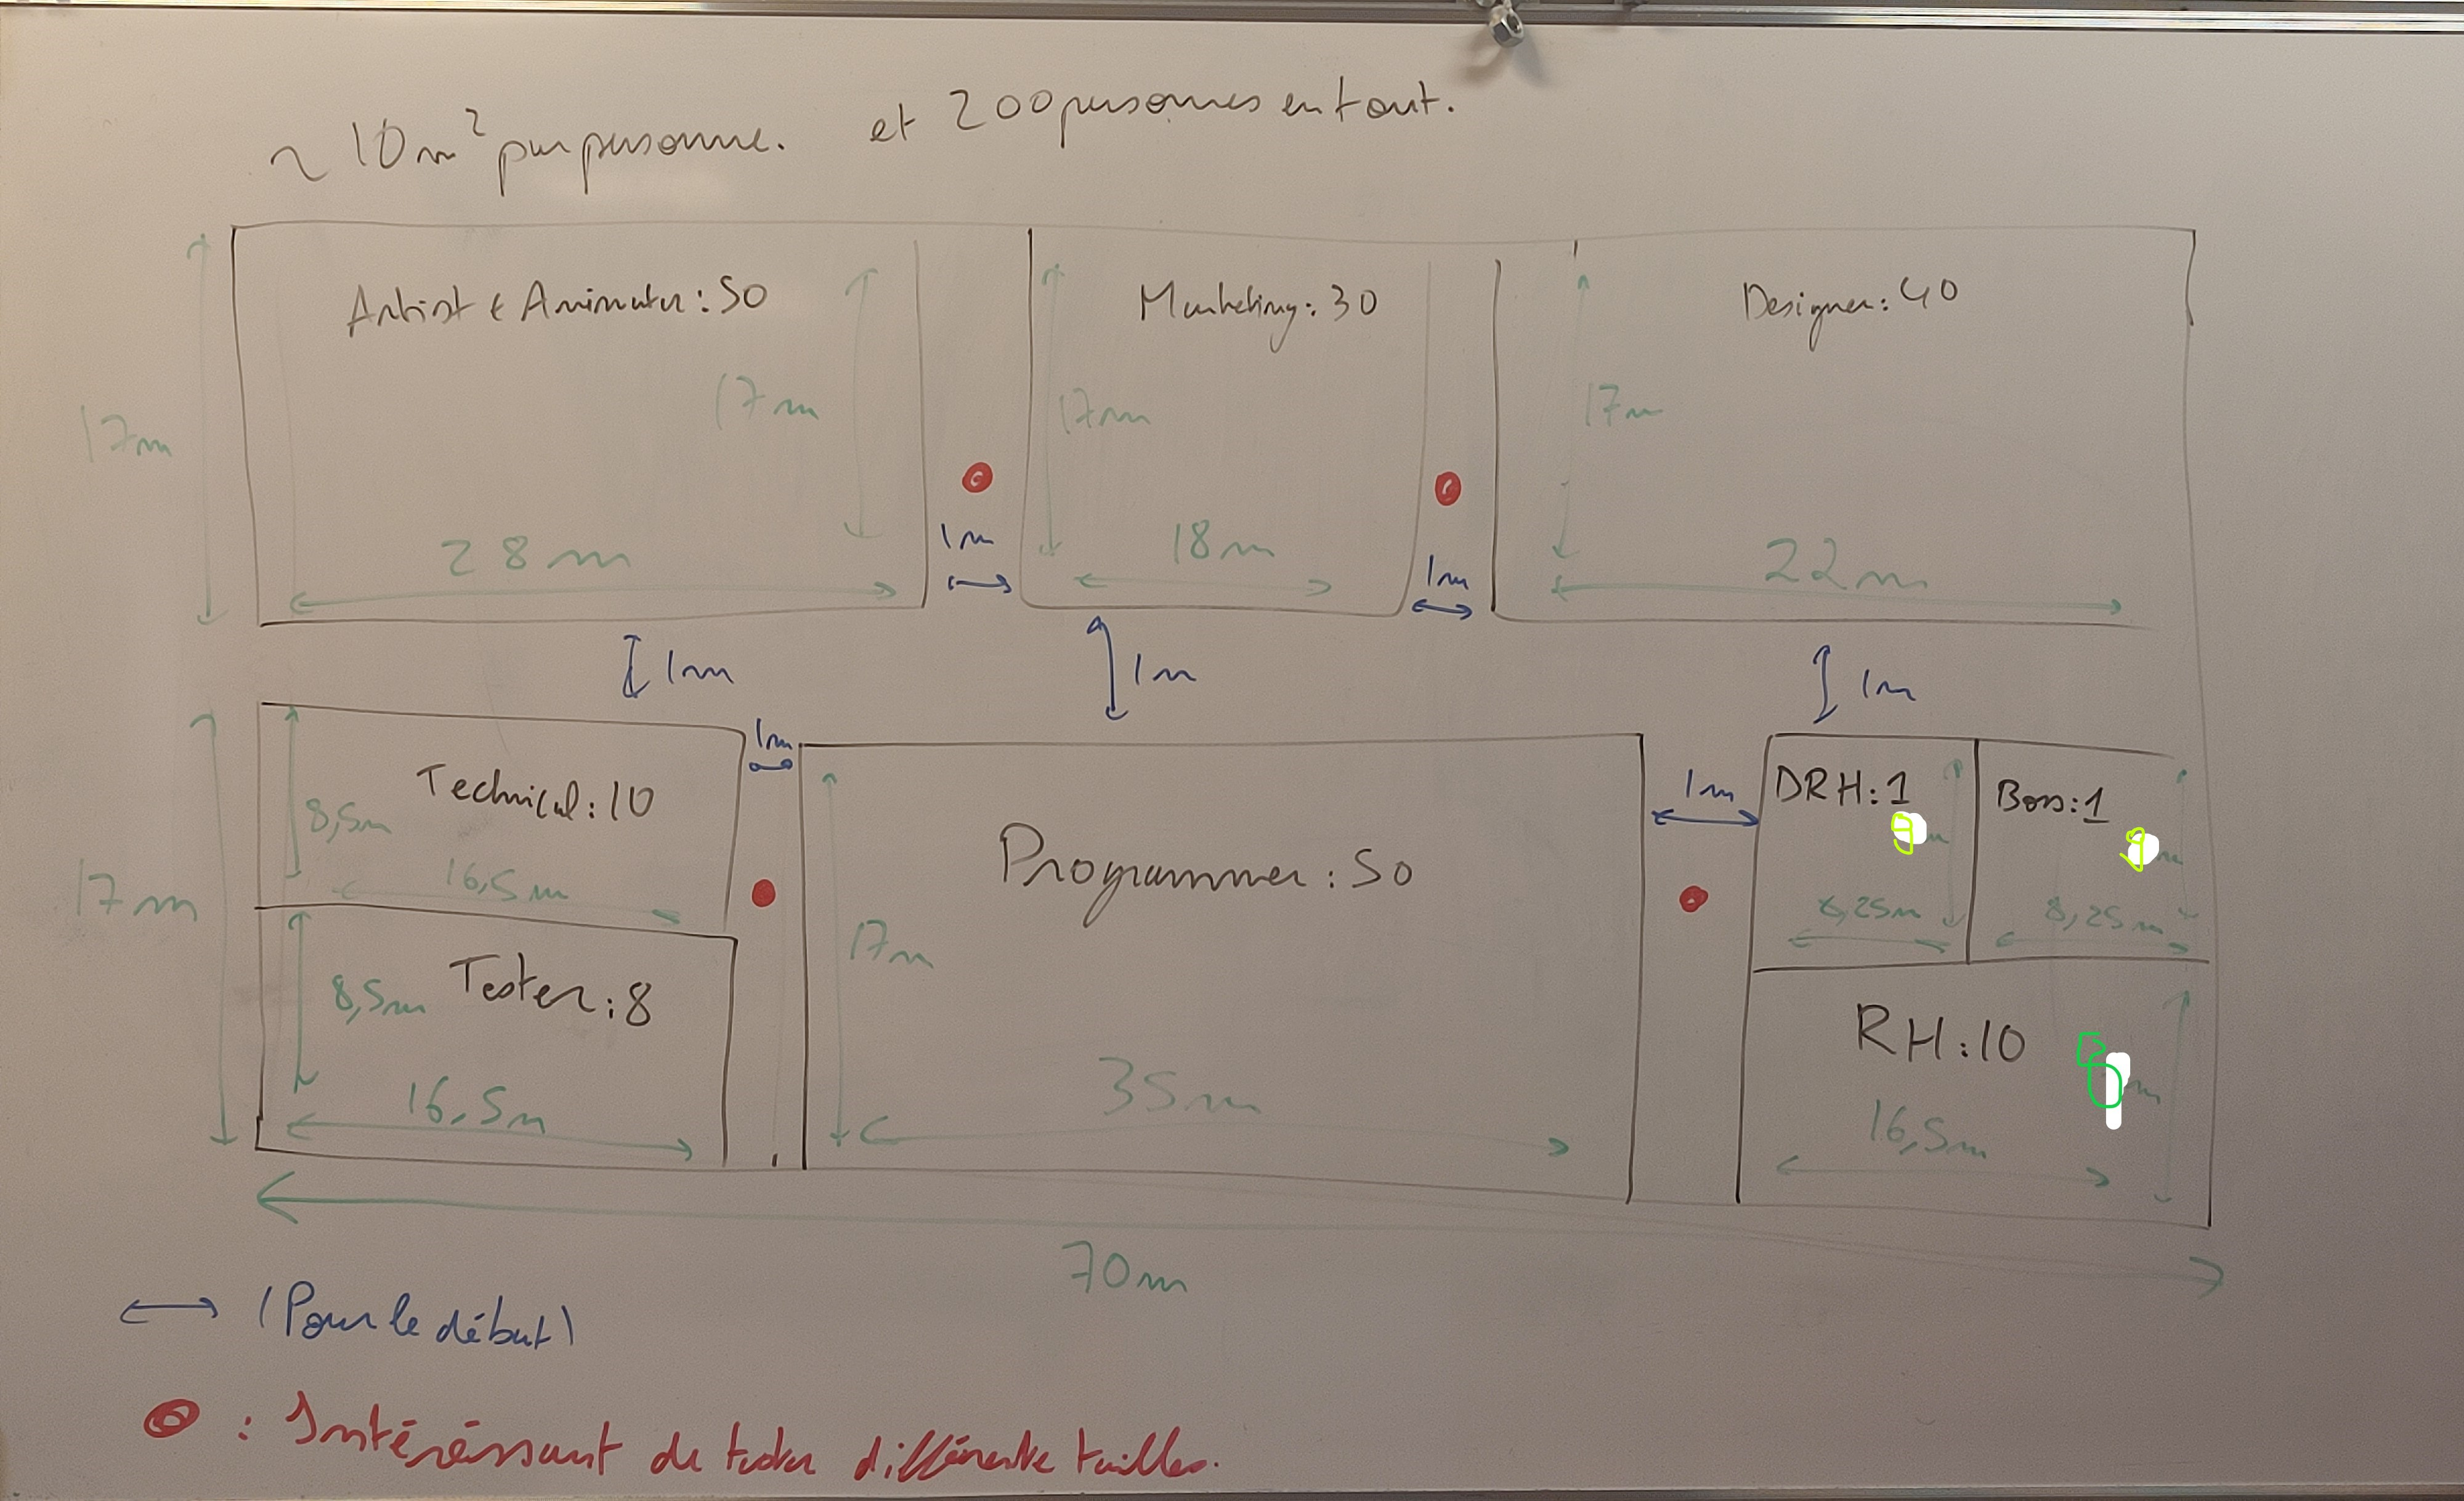
\includegraphics[scale=0.15]{Batiment optimisé croquis.jpg}
\newline\newline
Voici l'allure générale du bâtiment que je vais proposer d'optimiser.
\newline
Au départ il aura rien d'un bâtiment optmisé (couloir 1m, portes mauvais endroits...), mais 
on va montrer que grâce aux hypothèses validés on peut en effet diminuer le temps de sortie moyen.

\section{Premier Batiment}
On va reproduire le bâtiment sous sa forme non optimisé pour faire nos premières observations sur ce dernier.
\newline\newline
La photo ci-dessous montre le bâtiment dans sa phase originale (sans aucune optimisation et classique)
\end{document}